\scanpage{26}

% Local layout keeps the page references to the left of the long rule,
% and the two strong vertical rules beside/through the writing.
% The faint upper-left trace is reproduced without assigning a function.
\figure{\begin{tikzpicture}[x=.0084cm,y=-.0084cm,
  every node/.style={anchor=base west,inner sep=0pt,outer sep=0pt,font=\fontsize{9}{10.5}\selectfont}]
\draw[line width=.4pt] (234,93) -- (239,2343);
\draw[line width=.4pt] (1512,84) -- (1515,1230) -- (1523,2340);
\draw[gray!55,line width=.25pt] (54,120) -- (53,220) -- (58,272) -- (54,335) -- (58,385) -- (54,435) -- (58,483) -- (55,516) -- (58,574) -- (54,627) -- (58,691) -- (54,745) -- (58,810) -- (55,875) -- (58,945) -- (55,1010) -- (58,1080);
\node (top-text) at (265,105) {l.5 commutes with. l.18 is $C\overset{\inserted{=}}{\deleted{\unsure{\Rightarrow|\to}}}A$? confusing as it stands.};
\node[anchor=base east] (p276-reference) at (215,172) {276};
\node (p276-text) at (275,172) {l.15 ``equivalent to \deleted{\unsure{``}}$f$\tikz[baseline=(fq.base)]{\node[inner sep=0pt] (fq) {\deleted{\unsure{''}}};\draw[line width=.4pt] ([xshift=.1em,yshift=-1ex]fq.south west) -- ([xshift=.22em,yshift=-.65ex]fq.south west) -- ([xshift=.45em,yshift=-1.05ex]fq.south west);} commuting with'' !};
\node[anchor=base east] (p277-reference) at (215,235) {277};
\node (p277-text) at (265,235) {l.2 ``doesn't'' l-12 ``Of course''};
\node[anchor=base east] (p278-reference) at (215,300) {278};
\node (p278-text) at (265,300) {l-\deleted{\unsure{18}}17 ``definitely'' l-8 ``isn't'' l-5 ``we'd'' (i.e we had better assume)};
\node[anchor=base east] (p279-reference) at (215,365) {279};
\node (p279-text) at (265,365) {l11 ``didn't'' l-7 ``isn't''};
\node[anchor=base east] (p280-reference) at (215,425) {280};
\node (p280-text) at (270,425) {l-8 ``wasn't''};
\node[anchor=base east] (p281-reference) at (215,490) {281};
\node (p281-text) at (265,490) {l-11 ``which will allow us then...'' l-12 ``commutes with'' also in l-2.};
\node[anchor=base east] (p282-reference) at (215,550) {282};
\node (p282-text) at (275,550) {l.5 ``commutes with''};
\node[anchor=base east] (p283-reference) at (215,615) {283};
\node (p283-text) at (270,615) {l.2 ``commutes with'' also l.17 .. l17-18 ``doesn't'' + ``commutation...with''};
\node (p283b-text) at (285,680) {l-1 ``commutes with''};
\node[anchor=base east] (p284-reference) at (215,745) {284};
\node (p284-text) at (270,745) {l.3 ``commutation with'' l-9 ``commutes with\deleted{\unsure{''}}... and also with''};
\node[anchor=base east] (p285-reference) at (215,808) {285};
\node (p285-text) at (275,808) {l.9. ``commutes with''};
\node[anchor=base east] (p286-reference) at (215,872) {286};
\node (p286-text) at (275,872) {l15 ``its'' not ``it's'' (only used as abbrev. for ``it is''.)};
\node[anchor=base east] (p287-reference) at (215,934) {287};
\node (p287-text) at (275,934) {l.17 ``structure\tikz[baseline=(su.base)]{\node[inner sep=0pt] (su) {s};\draw[line width=.45pt] ([xshift=-.5pt,yshift=-1.5pt]su.south west) -- ([yshift=-1.5pt]su.south east) -- ([yshift=-3pt]su.south east) -- ([xshift=.5pt,yshift=-3pt]su.south west) -- ([xshift=.5pt,yshift=-4.5pt]su.south west) -- ([yshift=-4.5pt]su.south east);}''};
\node[anchor=base east] (p288-reference) at (215,998) {288};
\node (p288-text) at (275,998) {l.1 ``we've got'', The phrase ``hence .... $M'$. '' \deleted{d\unsure{o|e}} has no verb.};
\node (p288b-text) at (300,1063) {I suggest ``hence we have the sets etc''};
\node[anchor=base east] (p289-reference) at (215,1120) {289};
\node (p289-text) at (270,1120) {l-9 ``commute with'' l-8 ``with'' not ``to''};
\node[anchor=base east] (p290-reference) at (215,1183) {290};
\node (p290-text) at (275,1183) {l.2 ``isn't'' l.10 ``its''};
\node[anchor=base east] (p291-reference) at (215,1244) {p291};
\node (p291-text) at (265,1244) {l.1 ``couldn't'' l.9 ``hadn't'' l.10 ``to see what \deleted{pro} stronger property};
\node (p291b-text) at (285,1308) {to put in instead'' l15 'shouldn't''};
\node[anchor=base east] (p293-reference) at (215,1372) {p293};
\node (p293-text) at (275,1372) {l2. 'haven't'' l8 ``developed'' l15 ``didn't'' l-12 ``that I've got''};
\node (p293b-text) at (275,1438) {l-4 ``opposite'' \deleted{l\unsure{6}}, \deleted{Replace ``too'' by ``as well'' for \unsure{easier reading}}.};
\node (p293c-text) at (275,1505) {``too\deleted{''} in a natural way'' feels awkward. What about 'is so endowed};
\node (p293d-text) at (300,1567) {in any natural way.''};
\node[anchor=base east] (p294-reference) at (215,1626) {p294};
\node (p294-text) at (275,1626) {l13 ``make sense'' l-16 ``usual''};
\node[anchor=base east] (p295-reference) at (215,1692) {295};
\node (p295-text) at (265,1692) {l.16 ``where'' not \unsure{``|'}were''};
\node[anchor=base east] (p296-reference) at (215,1760) {296};
\node (p296-text) at (275,1760) {l.12 ``analogons'' isn't in the dictionary - ``analogues'' would work};
\node (p296b-text) at (280,1825) {l19 ``such a functor''};
\node[anchor=base east] (p297-reference) at (215,1887) {p.297};
\node (p297-text) at (275,1887) {l 1.1 ``developed''};
\node[anchor=base east] (p298-reference) at (215,1950) {298};
\node (p298-text) at (280,1950) {l.3 ``standard'' l-6 ``commutes with''};
\node[anchor=base east] (p299-reference) at (215,2012) {299};
\node (p299-text) at (275,2012) {l.3 ``commute with'' \& in l.4. l.16 'developed'' l.17 ``doesn't''};
\node (p299b-text) at (275,2075) {l20 ``its''};
\node[anchor=base east] (p300-reference) at (215,2137) {300};
\node (p300-text) at (275,2137) {l.4 ``don't'' l.11 delete ``the'' l.-15 ``doesn't''};
\node[anchor=base east] (p301-reference) at (215,2201) {301,};
\node (p301-text) at (280,2201) {l.-3 ``commute with''};
\node[anchor=base east] (p302-reference) at (215,2270) {302};
\node (p302-text) at (275,2270) {l.1. 'commute with \deleted{\unsure{''}} finite products and with'' l.5 ``commutation with''};
\end{tikzpicture}}

% archive sheet number: 25
